 %!TEX root = Projeto.tex
\section{Motivação}

% Contextualizar: o que está exposto no browser que deva ser protegido? Quais riscos?
A diversidade das aplicações disponíveis na web reflete a demanda de seus usuários por funcionalidade útil e interessante. A popularidade dessa plataforma denota o grau de confiança depositada pelos usuários em sua infraestrutura, ou não haveria procura pela utilização de serviços como comércio eletrônico, transações bancárias, redes sociais e troca de mensagens, para mencionar algumas das categorias de aplicações que fazem uso intensivo de dados pessoais, incluindo dados sigilosos ou de uso restrito.

A confiança com que os usuários interagem com a web, no entanto, é constantemente desafiada por falhas sistêmicas e ataques deliberados que culminam com o roubo e a adulteração das informações roteadas pelos diversos componentes que dão suporte às funcionalidades das aplicações web. Muitas vezes, o risco de vazamento de informação se manifesta justamente na ponta mais próxima do usuário: seu software navegador de internet. Ataques como o redirecionamento de \textit{scripts} em sites do \textit{bureau} de crédito norte-americano Equifax \cite{Segura2017}, a invasão e adulteração de scripts da rede de distribuição de conteúdo BootstrapCDN \cite{Dorfman2013}, a ousada exploração de \textit{malware} atingindo usuários do site E-Bay \cite{Vanunu2016}, e as divulgações recentes do comprometimento de extensões do aplicativo Chrome \cite{Forrest2017} apontam para vulnerabilidades intrínsecas nos recursos do navegador que dão suporte ao ``conteúdo ativo'', mecanismo essencial para as aplicações web interativas modernas \cite{Hedin2016}.

% Contextualizar: por que é importante um esforço para ajudar o desenvolvedor na proteção do conteúdo no navegador?
Assim, o desenvolvimento de uma aplicação segura para a web demanda esforços para que seja evitada a exposição e a manipulação indevidas das informações do usuário. Para esse propósito, o desenvolvedor conta com um conjunto de práticas e recomendações estabelecidas, efetivamente protegendo a aplicação e seus usuários de uma série de vulnerabilidades. Conjuntos de regras, como a SOP (\textit{same-origin policy}), e protocolos como o CORS (\textit{cross-origin resource sharing}) elevam a capacidade do navegador em manter um ambiente de execução seguro. Ambos se baseiam na noção do ``domínio'' como identificador da origem e, por consequência, da confiabilidade de um recurso: o domínio da página, denotado pela combinação do \textit{protocolo}, \textit{nome do host} e \textit{porta TCP} de onde o navegador requisitou o conteúdo carregado, é tido como o mais confiável, enquanto recursos requisitados de domínios diferentes são considerados menos confiáveis.
%CORS, por exemplo, foi destacado por \cite{DeRyck2012} em sua avaliação de mecanismos de segurança no navegador, na qual diversos dos mecanismos disponíveis são comparados segundo quatro categorias de requisitos -- Separação, Interação, Comunicação e Controle do Comportamento.

Contudo, tal ambiente é protegido dentro da condição de que todo conteúdo ativo carregado por uma aplicação está sob o conhecimento e confiança de seu desenvolvedor, o que nem sempre é o caso \cite{Heule2015_Most_Dangerous_Code}. Dentro da estrutura de documento da página web as informações dos usuários permanecem fundamentalmente expostas a \textit{scripts} mal-intencionados ou mal-escritos, executados em contexto da página ou como extensões do navegador. Criar um \textit{script} destinado a ler o conteúdo potencialmente sigiloso de uma página da web e revelá-lo a terceiros não autorizados é uma tarefa que exige pouca habilidade e que pode passar despercebida pelo aparato de segurança disponível, incluindo as restrições de SOP e CORS.

Código \textit{inline} ou \textit{scripts} baixados pelas páginas da web são executados com os mesmos privilégios e mesmo nível de acesso à estrutura de documento do navegador, o chamado DOM (\textit{document object model}) \cite[p. 2-3]{DeRyck2012}, não importando o domínio de origem dos scripts. Uma demonstração do problema pode ser exemplificada na figura \ref{Fig: diagrama01} e listagem de código \ref{Src: webPageMultiOrigin}. Nesse exemplo, um script tido como benigno é incorporado a uma página web a partir de um domínio de CDN (\textit{content delivery network}), diferente daquele da aplicação que efetivamente publica a página. O servidor da página, pelo protocolo CORS, sinaliza ao navegador que o domínio da CDN é confiável. O script externo pode, então, iniciar requisições ao seu domínio de origem -- uma consequência desejada pelos autores da página, pois o script depende desse acesso para efetuar suas funções.

\begin{figure}
	\centering
	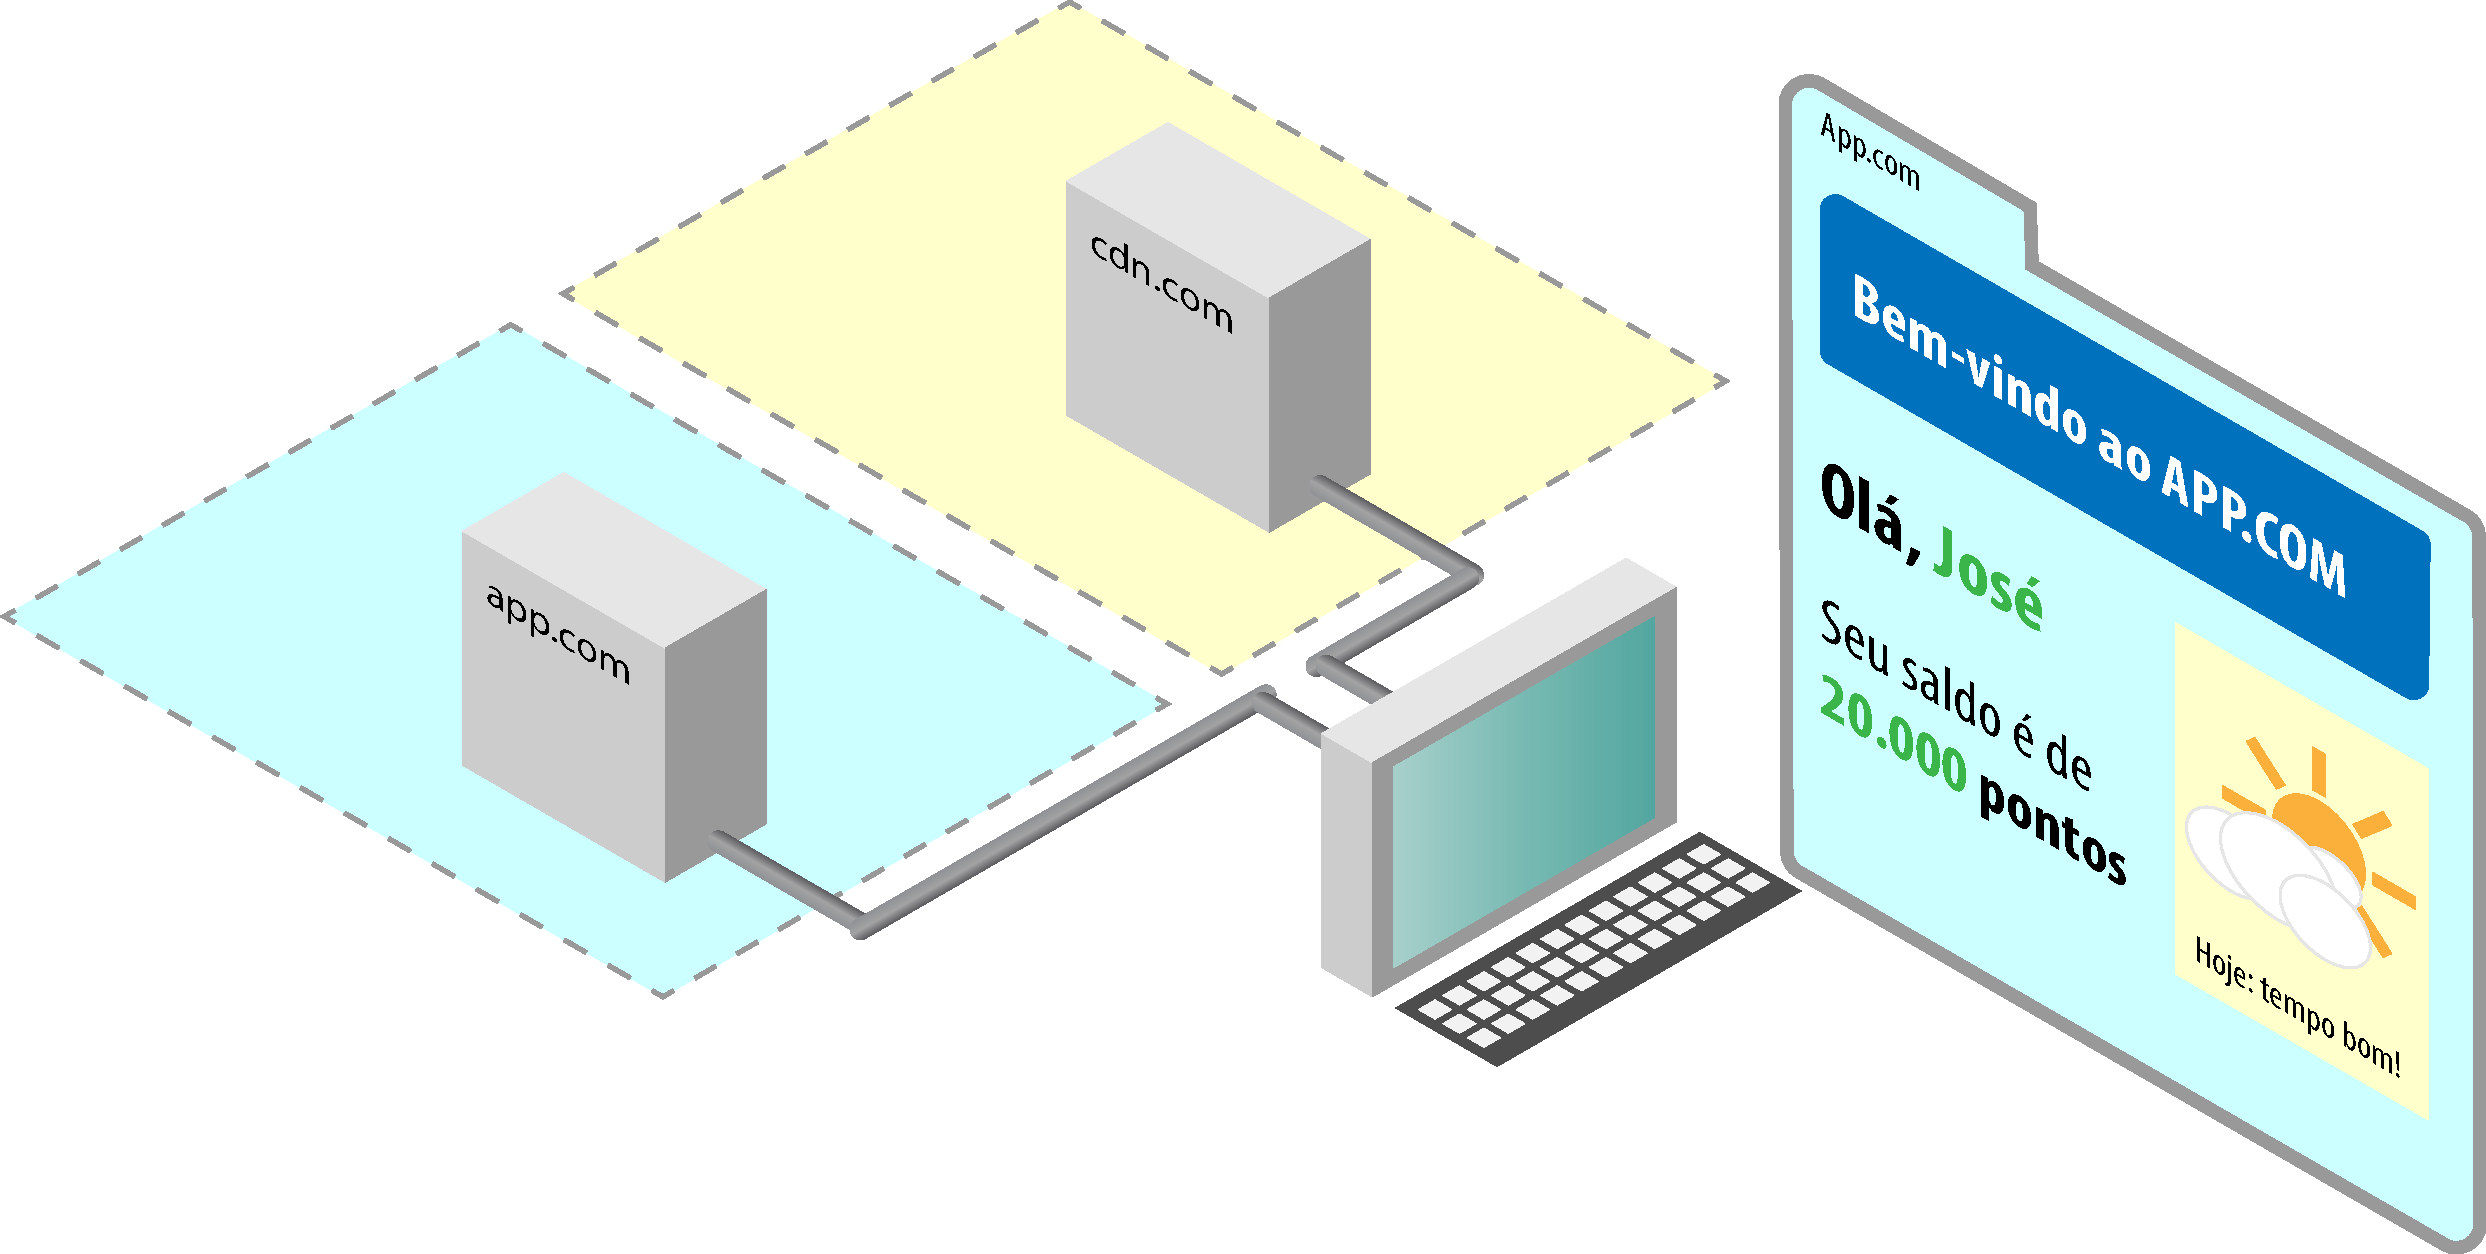
\includegraphics[width=15cm]{diagramas/diagrama01.pdf}
	\caption{Aplicação web composta por conteúdo proveniente de duas origens.}
	\label{Fig: diagrama01}
	
	\lstinputlisting[language=html,
		inputencoding=utf8,
		label={Src: webPageMultiOrigin},
		caption={[Página HTML incorporando script de outra origem]Incorporação de script de outra origem (linha \ref{lstCdnScript})}]{codigo/sample01-leaking-script.html}
\end{figure}

Em momento posterior, o script servido pelos servidores da CDN é substituído por código malicioso que, além de efetuar as funções do script benigno, captura o conteúdo da página armazenado no DOM. O script pode buscar informações específicas e potencialmente sensíveis como identificação do usuário, senhas e endereços. Por causa da autorização concedida pelo protocolo CORS, o código mal intencionado tem a chance de transmitir o conteúdo capturado para um serviço anômalo.

(DIAGRAMA 2: COMPORTAMENTO DA APLICAÇÃO APÓS A PUBLICAÇÃO DO SCRIPT MALICIOSO)

Acessar, capturar e modificar informações contidas no DOM também são efeitos de extensões do navegador. Mas, diferentemente dos scripts incorporados em páginas, extensões são executadas em modo privilegiado e podem afetar todas as páginas carregadas pelo navegador, não sendo confinadas a domínios específicos. Extensões como as do Google Chrome são publicadas exclusivamente em site específico e protegido, mas não é impossível que o código fonte de extensões seja descaracterizado e publicado pela ação de \textit{hackers} \cite{Spring2017}, afetando a todos os usuários que atualizarem a extensão -- um processo automático por padrão \cite{Google2017}. 

(DIAGRAMA 3: AÇÃO DE UMA EXTENSÃO COMPROMETIDA)

% Contextualizar: o que tem sido feito nessa direção, em termos de padrões estabelecidos?
%Na raiz das vulnerabilidades está a forma inconsistente e parcial com que a linguagem Javascript e as APIs do navegador tratam o isolamento entre \textit{scripts} e dados. 
%Vulnerabilidades têm se manifestado desde o momento em que os navegadores e servidores passaram a dar suporte a \textit{cookies}, à linguagem Javascript, ao DOM e aos recursos de incorporação de mídia, porém as formas de mitigação dessas vulnerabilidades competem entre si e com as funcionalidades de que os desenvolvedores dependem, resultando em regras e práticas inconsistentes e incompletas \cite{Hill2016}.



%Segundo Foster1998, a segurança da infraestrutura de internet se baseia em duas classes de serviço: (1) serviços de controle de acesso e (2) serviços de segurança da comunicação.

% Contextualizar: o que tem sido feito nessa direção, em termos de experimentos?
(Contextualizar: o que tem sido feito nessa direção, em termos de experimentos?)
%Na raiz das vulnerabilidades está a forma inconsistente e parcial com que a linguagem Javascript e as APIs do navegador tratam o isolamento entre \textit{scripts} e dados. A caracterização e a solução desse problema fazem parte de um campo de pesquisas ativo \cite{Stefan2014}, \cite{Hedin2014}, \cite{Bichhawat2014}, \cite{Magazinius2014} e em busca por padronização \cite{W3C:WebAppSec}, mas que ainda não resultou em práticas, ferramentas e protocolos de amplo alcance pois dependem da adoção de políticas de segurança experimentais \cite{Hedin2014}, \cite{Bichhawat2014} e potencialmente degradantes de desempenho \cite[p. 14]{Stefan2014} por parte dos desenvolvedores de navegadores.

%No campo das tecnologias experimentais estão as estratégias baseadas no controle do fluxo da informação (IFC, \textit{information flow control}). IFC, inicialmente descrito por \cite{Denning1976}, estabelece que cada espaço de armazenamento em um programa -- arquivos, segmentos de memória, conexões de rede ou variáveis, por exemplo -- seja rotulado por uma classe de segurança. Em função disso, o trânsito de informação entre espaços de armazenamento deve ser monitorado e, eventualmente, interrompido quando os rótulos da origem e do destino da informação não forem compatíveis. IFC é um mecanismo inexistente nas implementações da linguagem Javascript dos navegadores da web; implementá-lo em uma linguagem dinâmica como Javascript significa introduzir uma checagem de rótulos a cada leitura e escrita em objetos mutáveis \cite[p.3]{Heule2015_IFC_Inside}, acarretando perdas significativas na velocidade da execução de \textit{scripts}.

% Contextualizar: como esta proposta contribui?
(Contextualizar: como esta proposta contribui?)



%Na web, o desafio de transmitir dados sensíveis com integridade e confidencialidade envolve a colaboração entre todos os contextos em que esses dados possam transitar: sistemas de \textit{backend}, bancos de dados e servidores de aplicação, a rede entre os \textit{hosts} participantes, o modelo de documento da HTML (DOM), os \textit{scripts} carregados pelas páginas web, e e o próprio ambiente de execução do navegador, incluindo suas extensões e \textit{plugins}. Ainda que possível, garantir segurança no fluxo da informação entre esses contextos não é algo ao alcance do desenvolvedor de aplicações. 




